
\documentclass{article} % For LaTeX2e
\usepackage{iclr2027_conference,times}

% Optional math commands from https://github.com/goodfeli/dlbook_notation.
%%%%% NEW MATH DEFINITIONS %%%%%

\usepackage{amsmath,amsfonts,bm}

% Mark sections of captions for referring to divisions of figures
\newcommand{\figleft}{{\em (Left)}}
\newcommand{\figcenter}{{\em (Center)}}
\newcommand{\figright}{{\em (Right)}}
\newcommand{\figtop}{{\em (Top)}}
\newcommand{\figbottom}{{\em (Bottom)}}
\newcommand{\captiona}{{\em (a)}}
\newcommand{\captionb}{{\em (b)}}
\newcommand{\captionc}{{\em (c)}}
\newcommand{\captiond}{{\em (d)}}

% Highlight a newly defined term
\newcommand{\newterm}[1]{{\bf #1}}


% Figure reference, lower-case.
\def\figref#1{figure~\ref{#1}}
% Figure reference, capital. For start of sentence
\def\Figref#1{Figure~\ref{#1}}
\def\twofigref#1#2{figures \ref{#1} and \ref{#2}}
\def\quadfigref#1#2#3#4{figures \ref{#1}, \ref{#2}, \ref{#3} and \ref{#4}}
% Section reference, lower-case.
\def\secref#1{section~\ref{#1}}
% Section reference, capital.
\def\Secref#1{Section~\ref{#1}}
% Reference to two sections.
\def\twosecrefs#1#2{sections \ref{#1} and \ref{#2}}
% Reference to three sections.
\def\secrefs#1#2#3{sections \ref{#1}, \ref{#2} and \ref{#3}}
% Reference to an equation, lower-case.
\def\eqref#1{equation~\ref{#1}}
% Reference to an equation, upper case
\def\Eqref#1{Equation~\ref{#1}}
% A raw reference to an equation---avoid using if possible
\def\plaineqref#1{\ref{#1}}
% Reference to a chapter, lower-case.
\def\chapref#1{chapter~\ref{#1}}
% Reference to an equation, upper case.
\def\Chapref#1{Chapter~\ref{#1}}
% Reference to a range of chapters
\def\rangechapref#1#2{chapters\ref{#1}--\ref{#2}}
% Reference to an algorithm, lower-case.
\def\algref#1{algorithm~\ref{#1}}
% Reference to an algorithm, upper case.
\def\Algref#1{Algorithm~\ref{#1}}
\def\twoalgref#1#2{algorithms \ref{#1} and \ref{#2}}
\def\Twoalgref#1#2{Algorithms \ref{#1} and \ref{#2}}
% Reference to a part, lower case
\def\partref#1{part~\ref{#1}}
% Reference to a part, upper case
\def\Partref#1{Part~\ref{#1}}
\def\twopartref#1#2{parts \ref{#1} and \ref{#2}}

\def\ceil#1{\lceil #1 \rceil}
\def\floor#1{\lfloor #1 \rfloor}
\def\1{\bm{1}}
\newcommand{\train}{\mathcal{D}}
\newcommand{\valid}{\mathcal{D_{\mathrm{valid}}}}
\newcommand{\test}{\mathcal{D_{\mathrm{test}}}}

\def\eps{{\epsilon}}


% Random variables
\def\reta{{\textnormal{$\eta$}}}
\def\ra{{\textnormal{a}}}
\def\rb{{\textnormal{b}}}
\def\rc{{\textnormal{c}}}
\def\rd{{\textnormal{d}}}
\def\re{{\textnormal{e}}}
\def\rf{{\textnormal{f}}}
\def\rg{{\textnormal{g}}}
\def\rh{{\textnormal{h}}}
\def\ri{{\textnormal{i}}}
\def\rj{{\textnormal{j}}}
\def\rk{{\textnormal{k}}}
\def\rl{{\textnormal{l}}}
% rm is already a command, just don't name any random variables m
\def\rn{{\textnormal{n}}}
\def\ro{{\textnormal{o}}}
\def\rp{{\textnormal{p}}}
\def\rq{{\textnormal{q}}}
\def\rr{{\textnormal{r}}}
\def\rs{{\textnormal{s}}}
\def\rt{{\textnormal{t}}}
\def\ru{{\textnormal{u}}}
\def\rv{{\textnormal{v}}}
\def\rw{{\textnormal{w}}}
\def\rx{{\textnormal{x}}}
\def\ry{{\textnormal{y}}}
\def\rz{{\textnormal{z}}}

% Random vectors
\def\rvepsilon{{\mathbf{\epsilon}}}
\def\rvtheta{{\mathbf{\theta}}}
\def\rva{{\mathbf{a}}}
\def\rvb{{\mathbf{b}}}
\def\rvc{{\mathbf{c}}}
\def\rvd{{\mathbf{d}}}
\def\rve{{\mathbf{e}}}
\def\rvf{{\mathbf{f}}}
\def\rvg{{\mathbf{g}}}
\def\rvh{{\mathbf{h}}}
\def\rvu{{\mathbf{i}}}
\def\rvj{{\mathbf{j}}}
\def\rvk{{\mathbf{k}}}
\def\rvl{{\mathbf{l}}}
\def\rvm{{\mathbf{m}}}
\def\rvn{{\mathbf{n}}}
\def\rvo{{\mathbf{o}}}
\def\rvp{{\mathbf{p}}}
\def\rvq{{\mathbf{q}}}
\def\rvr{{\mathbf{r}}}
\def\rvs{{\mathbf{s}}}
\def\rvt{{\mathbf{t}}}
\def\rvu{{\mathbf{u}}}
\def\rvv{{\mathbf{v}}}
\def\rvw{{\mathbf{w}}}
\def\rvx{{\mathbf{x}}}
\def\rvy{{\mathbf{y}}}
\def\rvz{{\mathbf{z}}}

% Elements of random vectors
\def\erva{{\textnormal{a}}}
\def\ervb{{\textnormal{b}}}
\def\ervc{{\textnormal{c}}}
\def\ervd{{\textnormal{d}}}
\def\erve{{\textnormal{e}}}
\def\ervf{{\textnormal{f}}}
\def\ervg{{\textnormal{g}}}
\def\ervh{{\textnormal{h}}}
\def\ervi{{\textnormal{i}}}
\def\ervj{{\textnormal{j}}}
\def\ervk{{\textnormal{k}}}
\def\ervl{{\textnormal{l}}}
\def\ervm{{\textnormal{m}}}
\def\ervn{{\textnormal{n}}}
\def\ervo{{\textnormal{o}}}
\def\ervp{{\textnormal{p}}}
\def\ervq{{\textnormal{q}}}
\def\ervr{{\textnormal{r}}}
\def\ervs{{\textnormal{s}}}
\def\ervt{{\textnormal{t}}}
\def\ervu{{\textnormal{u}}}
\def\ervv{{\textnormal{v}}}
\def\ervw{{\textnormal{w}}}
\def\ervx{{\textnormal{x}}}
\def\ervy{{\textnormal{y}}}
\def\ervz{{\textnormal{z}}}

% Random matrices
\def\rmA{{\mathbf{A}}}
\def\rmB{{\mathbf{B}}}
\def\rmC{{\mathbf{C}}}
\def\rmD{{\mathbf{D}}}
\def\rmE{{\mathbf{E}}}
\def\rmF{{\mathbf{F}}}
\def\rmG{{\mathbf{G}}}
\def\rmH{{\mathbf{H}}}
\def\rmI{{\mathbf{I}}}
\def\rmJ{{\mathbf{J}}}
\def\rmK{{\mathbf{K}}}
\def\rmL{{\mathbf{L}}}
\def\rmM{{\mathbf{M}}}
\def\rmN{{\mathbf{N}}}
\def\rmO{{\mathbf{O}}}
\def\rmP{{\mathbf{P}}}
\def\rmQ{{\mathbf{Q}}}
\def\rmR{{\mathbf{R}}}
\def\rmS{{\mathbf{S}}}
\def\rmT{{\mathbf{T}}}
\def\rmU{{\mathbf{U}}}
\def\rmV{{\mathbf{V}}}
\def\rmW{{\mathbf{W}}}
\def\rmX{{\mathbf{X}}}
\def\rmY{{\mathbf{Y}}}
\def\rmZ{{\mathbf{Z}}}

% Elements of random matrices
\def\ermA{{\textnormal{A}}}
\def\ermB{{\textnormal{B}}}
\def\ermC{{\textnormal{C}}}
\def\ermD{{\textnormal{D}}}
\def\ermE{{\textnormal{E}}}
\def\ermF{{\textnormal{F}}}
\def\ermG{{\textnormal{G}}}
\def\ermH{{\textnormal{H}}}
\def\ermI{{\textnormal{I}}}
\def\ermJ{{\textnormal{J}}}
\def\ermK{{\textnormal{K}}}
\def\ermL{{\textnormal{L}}}
\def\ermM{{\textnormal{M}}}
\def\ermN{{\textnormal{N}}}
\def\ermO{{\textnormal{O}}}
\def\ermP{{\textnormal{P}}}
\def\ermQ{{\textnormal{Q}}}
\def\ermR{{\textnormal{R}}}
\def\ermS{{\textnormal{S}}}
\def\ermT{{\textnormal{T}}}
\def\ermU{{\textnormal{U}}}
\def\ermV{{\textnormal{V}}}
\def\ermW{{\textnormal{W}}}
\def\ermX{{\textnormal{X}}}
\def\ermY{{\textnormal{Y}}}
\def\ermZ{{\textnormal{Z}}}

% Vectors
\def\vzero{{\bm{0}}}
\def\vone{{\bm{1}}}
\def\vmu{{\bm{\mu}}}
\def\vtheta{{\bm{\theta}}}
\def\va{{\bm{a}}}
\def\vb{{\bm{b}}}
\def\vc{{\bm{c}}}
\def\vd{{\bm{d}}}
\def\ve{{\bm{e}}}
\def\vf{{\bm{f}}}
\def\vg{{\bm{g}}}
\def\vh{{\bm{h}}}
\def\vi{{\bm{i}}}
\def\vj{{\bm{j}}}
\def\vk{{\bm{k}}}
\def\vl{{\bm{l}}}
\def\vm{{\bm{m}}}
\def\vn{{\bm{n}}}
\def\vo{{\bm{o}}}
\def\vp{{\bm{p}}}
\def\vq{{\bm{q}}}
\def\vr{{\bm{r}}}
\def\vs{{\bm{s}}}
\def\vt{{\bm{t}}}
\def\vu{{\bm{u}}}
\def\vv{{\bm{v}}}
\def\vw{{\bm{w}}}
\def\vx{{\bm{x}}}
\def\vy{{\bm{y}}}
\def\vz{{\bm{z}}}

% Elements of vectors
\def\evalpha{{\alpha}}
\def\evbeta{{\beta}}
\def\evepsilon{{\epsilon}}
\def\evlambda{{\lambda}}
\def\evomega{{\omega}}
\def\evmu{{\mu}}
\def\evpsi{{\psi}}
\def\evsigma{{\sigma}}
\def\evtheta{{\theta}}
\def\eva{{a}}
\def\evb{{b}}
\def\evc{{c}}
\def\evd{{d}}
\def\eve{{e}}
\def\evf{{f}}
\def\evg{{g}}
\def\evh{{h}}
\def\evi{{i}}
\def\evj{{j}}
\def\evk{{k}}
\def\evl{{l}}
\def\evm{{m}}
\def\evn{{n}}
\def\evo{{o}}
\def\evp{{p}}
\def\evq{{q}}
\def\evr{{r}}
\def\evs{{s}}
\def\evt{{t}}
\def\evu{{u}}
\def\evv{{v}}
\def\evw{{w}}
\def\evx{{x}}
\def\evy{{y}}
\def\evz{{z}}

% Matrix
\def\mA{{\bm{A}}}
\def\mB{{\bm{B}}}
\def\mC{{\bm{C}}}
\def\mD{{\bm{D}}}
\def\mE{{\bm{E}}}
\def\mF{{\bm{F}}}
\def\mG{{\bm{G}}}
\def\mH{{\bm{H}}}
\def\mI{{\bm{I}}}
\def\mJ{{\bm{J}}}
\def\mK{{\bm{K}}}
\def\mL{{\bm{L}}}
\def\mM{{\bm{M}}}
\def\mN{{\bm{N}}}
\def\mO{{\bm{O}}}
\def\mP{{\bm{P}}}
\def\mQ{{\bm{Q}}}
\def\mR{{\bm{R}}}
\def\mS{{\bm{S}}}
\def\mT{{\bm{T}}}
\def\mU{{\bm{U}}}
\def\mV{{\bm{V}}}
\def\mW{{\bm{W}}}
\def\mX{{\bm{X}}}
\def\mY{{\bm{Y}}}
\def\mZ{{\bm{Z}}}
\def\mBeta{{\bm{\beta}}}
\def\mPhi{{\bm{\Phi}}}
\def\mLambda{{\bm{\Lambda}}}
\def\mSigma{{\bm{\Sigma}}}

% Tensor
\DeclareMathAlphabet{\mathsfit}{\encodingdefault}{\sfdefault}{m}{sl}
\SetMathAlphabet{\mathsfit}{bold}{\encodingdefault}{\sfdefault}{bx}{n}
\newcommand{\tens}[1]{\bm{\mathsfit{#1}}}
\def\tA{{\tens{A}}}
\def\tB{{\tens{B}}}
\def\tC{{\tens{C}}}
\def\tD{{\tens{D}}}
\def\tE{{\tens{E}}}
\def\tF{{\tens{F}}}
\def\tG{{\tens{G}}}
\def\tH{{\tens{H}}}
\def\tI{{\tens{I}}}
\def\tJ{{\tens{J}}}
\def\tK{{\tens{K}}}
\def\tL{{\tens{L}}}
\def\tM{{\tens{M}}}
\def\tN{{\tens{N}}}
\def\tO{{\tens{O}}}
\def\tP{{\tens{P}}}
\def\tQ{{\tens{Q}}}
\def\tR{{\tens{R}}}
\def\tS{{\tens{S}}}
\def\tT{{\tens{T}}}
\def\tU{{\tens{U}}}
\def\tV{{\tens{V}}}
\def\tW{{\tens{W}}}
\def\tX{{\tens{X}}}
\def\tY{{\tens{Y}}}
\def\tZ{{\tens{Z}}}


% Graph
\def\gA{{\mathcal{A}}}
\def\gB{{\mathcal{B}}}
\def\gC{{\mathcal{C}}}
\def\gD{{\mathcal{D}}}
\def\gE{{\mathcal{E}}}
\def\gF{{\mathcal{F}}}
\def\gG{{\mathcal{G}}}
\def\gH{{\mathcal{H}}}
\def\gI{{\mathcal{I}}}
\def\gJ{{\mathcal{J}}}
\def\gK{{\mathcal{K}}}
\def\gL{{\mathcal{L}}}
\def\gM{{\mathcal{M}}}
\def\gN{{\mathcal{N}}}
\def\gO{{\mathcal{O}}}
\def\gP{{\mathcal{P}}}
\def\gQ{{\mathcal{Q}}}
\def\gR{{\mathcal{R}}}
\def\gS{{\mathcal{S}}}
\def\gT{{\mathcal{T}}}
\def\gU{{\mathcal{U}}}
\def\gV{{\mathcal{V}}}
\def\gW{{\mathcal{W}}}
\def\gX{{\mathcal{X}}}
\def\gY{{\mathcal{Y}}}
\def\gZ{{\mathcal{Z}}}

% Sets
\def\sA{{\mathbb{A}}}
\def\sB{{\mathbb{B}}}
\def\sC{{\mathbb{C}}}
\def\sD{{\mathbb{D}}}
% Don't use a set called E, because this would be the same as our symbol
% for expectation.
\def\sF{{\mathbb{F}}}
\def\sG{{\mathbb{G}}}
\def\sH{{\mathbb{H}}}
\def\sI{{\mathbb{I}}}
\def\sJ{{\mathbb{J}}}
\def\sK{{\mathbb{K}}}
\def\sL{{\mathbb{L}}}
\def\sM{{\mathbb{M}}}
\def\sN{{\mathbb{N}}}
\def\sO{{\mathbb{O}}}
\def\sP{{\mathbb{P}}}
\def\sQ{{\mathbb{Q}}}
\def\sR{{\mathbb{R}}}
\def\sS{{\mathbb{S}}}
\def\sT{{\mathbb{T}}}
\def\sU{{\mathbb{U}}}
\def\sV{{\mathbb{V}}}
\def\sW{{\mathbb{W}}}
\def\sX{{\mathbb{X}}}
\def\sY{{\mathbb{Y}}}
\def\sZ{{\mathbb{Z}}}

% Entries of a matrix
\def\emLambda{{\Lambda}}
\def\emA{{A}}
\def\emB{{B}}
\def\emC{{C}}
\def\emD{{D}}
\def\emE{{E}}
\def\emF{{F}}
\def\emG{{G}}
\def\emH{{H}}
\def\emI{{I}}
\def\emJ{{J}}
\def\emK{{K}}
\def\emL{{L}}
\def\emM{{M}}
\def\emN{{N}}
\def\emO{{O}}
\def\emP{{P}}
\def\emQ{{Q}}
\def\emR{{R}}
\def\emS{{S}}
\def\emT{{T}}
\def\emU{{U}}
\def\emV{{V}}
\def\emW{{W}}
\def\emX{{X}}
\def\emY{{Y}}
\def\emZ{{Z}}
\def\emSigma{{\Sigma}}

% entries of a tensor
% Same font as tensor, without \bm wrapper
\newcommand{\etens}[1]{\mathsfit{#1}}
\def\etLambda{{\etens{\Lambda}}}
\def\etA{{\etens{A}}}
\def\etB{{\etens{B}}}
\def\etC{{\etens{C}}}
\def\etD{{\etens{D}}}
\def\etE{{\etens{E}}}
\def\etF{{\etens{F}}}
\def\etG{{\etens{G}}}
\def\etH{{\etens{H}}}
\def\etI{{\etens{I}}}
\def\etJ{{\etens{J}}}
\def\etK{{\etens{K}}}
\def\etL{{\etens{L}}}
\def\etM{{\etens{M}}}
\def\etN{{\etens{N}}}
\def\etO{{\etens{O}}}
\def\etP{{\etens{P}}}
\def\etQ{{\etens{Q}}}
\def\etR{{\etens{R}}}
\def\etS{{\etens{S}}}
\def\etT{{\etens{T}}}
\def\etU{{\etens{U}}}
\def\etV{{\etens{V}}}
\def\etW{{\etens{W}}}
\def\etX{{\etens{X}}}
\def\etY{{\etens{Y}}}
\def\etZ{{\etens{Z}}}

% The true underlying data generating distribution
\newcommand{\pdata}{p_{\rm{data}}}
% The empirical distribution defined by the training set
\newcommand{\ptrain}{\hat{p}_{\rm{data}}}
\newcommand{\Ptrain}{\hat{P}_{\rm{data}}}
% The model distribution
\newcommand{\pmodel}{p_{\rm{model}}}
\newcommand{\Pmodel}{P_{\rm{model}}}
\newcommand{\ptildemodel}{\tilde{p}_{\rm{model}}}
% Stochastic autoencoder distributions
\newcommand{\pencode}{p_{\rm{encoder}}}
\newcommand{\pdecode}{p_{\rm{decoder}}}
\newcommand{\precons}{p_{\rm{reconstruct}}}

\newcommand{\laplace}{\mathrm{Laplace}} % Laplace distribution

\newcommand{\E}{\mathbb{E}}
\newcommand{\Ls}{\mathcal{L}}
\newcommand{\R}{\mathbb{R}}
\newcommand{\emp}{\tilde{p}}
\newcommand{\lr}{\alpha}
\newcommand{\reg}{\lambda}
\newcommand{\rect}{\mathrm{rectifier}}
\newcommand{\softmax}{\mathrm{softmax}}
\newcommand{\sigmoid}{\sigma}
\newcommand{\softplus}{\zeta}
\newcommand{\KL}{D_{\mathrm{KL}}}
\newcommand{\Var}{\mathrm{Var}}
\newcommand{\standarderror}{\mathrm{SE}}
\newcommand{\Cov}{\mathrm{Cov}}
% Wolfram Mathworld says $L^2$ is for function spaces and $\ell^2$ is for vectors
% But then they seem to use $L^2$ for vectors throughout the site, and so does
% wikipedia.
\newcommand{\normlzero}{L^0}
\newcommand{\normlone}{L^1}
\newcommand{\normltwo}{L^2}
\newcommand{\normlp}{L^p}
\newcommand{\normmax}{L^\infty}

\newcommand{\parents}{Pa} % See usage in notation.tex. Chosen to match Daphne's book.

\DeclareMathOperator*{\argmax}{arg\,max}
\DeclareMathOperator*{\argmin}{arg\,min}

\DeclareMathOperator{\sign}{sign}
\DeclareMathOperator{\Tr}{Tr}
\let\ab\allowbreak


\usepackage{hyperref}
\usepackage{url}
\usepackage{graphicx}
\usepackage{wrapfig}


\title{Physics-Informed Training at the Operator Level}

% Authors must not appear in the submitted version. They should be hidden
% as long as the \iclrfinalcopy macro remains commented out below.
% Non-anonymous submissions will be rejected without review.

\author{
Shizheng Wen\thanks{Equal contribution.} \\
ETH Zürich \\
\texttt{shizheng.wen@math.ethz.ch}
\And
Marius Zeinhofer\footnotemark[1] \\
ETH Zürich \\
\texttt{marius.zeinhofer@math.ethz.ch}
\And
Siddhartha Mishra \\
ETH Zürich \\
\texttt{siddhartha.mishra@math.ethz.ch}
}

% The \author macro works with any number of authors. There are two commands
% used to separate the names and addresses of multiple authors: \And and \AND.
%
% Using \And between authors leaves it to \LaTeX{} to determine where to break
% the lines. Using \AND forces a linebreak at that point. So, if \LaTeX{}
% puts 3 of 4 authors names on the first line, and the last on the second
% line, try using \AND instead of \And before the third author name.

\newcommand{\fix}{\marginpar{FIX}}
\newcommand{\new}{\marginpar{NEW}}

%\iclrfinalcopy % Uncomment for camera-ready version, but NOT for submission.
\begin{document}


\maketitle

\begin{abstract}
   We present an approach to train neural operators physics-informed, i.e., in a self-supervised fashion, purely relying on the governing physical equations. This enables training on infinite datasets where no sample is visited twice and removes the need to produce training data in an offline phase. While previous attempts for physics-informed training at the operator level were limited to benign problems and performed considerably worse than data-driven learning, our approach matches the gold-standard of data-driven training at a similar optimization cost. Our method is based on modifying the physics-informed loss functions to include a preconditioner such as a multigrid method to drastically reduce the ill-conditioning caused by unbounded PDE operators. We derive the improved conditioning theoretically, and illustrate the potential of the method for the Poisson, Allen-Cahn, and stationary Stokes equation, where it performs virtually identical to data-driven training at a comparable computational cost.
\end{abstract}

\section{Introduction}

% Importance of fast solutions of PDEs. A tool for this in the age of AI: neural operators
\paragraph{Neural Operators}
Despite a century of development of numerical methods, partial differential equations (PDEs) remain expensive to solve, even more so in many-query situations, such as uncertainty quantification, optimal control, and inverse problems. The development of fast PDE solution techniques, e.g., through reduced-order/surrogate models therefore is of utmost importance. In the wake of the deep learning revolution, neural operators emerged as a powerful computational tool for surrogate modeling, drastically reducing PDE solution time in many applications. Neural operators approximate maps between infinite-dimensional spaces (operators) by a neural network, and are typically trained in a supervised fashion. They hence require a dataset that is built in an offline fashion, before they can be trained, and eventually used downstream. Data generation can constitute a substantial part of the computation and engineering effort, even more so in the context of physics foundation models that are pre-trained over an array of different PDE instances.

% Declared here, after the text that fills page 1, so [t] places it at the top of page 2.
% Regenerate with
%   python experiments/graphical_abstract/plot_abstract.py \
%       --bare output/graphical_abstract/abstract_v1/bare.npz \
%       --mg   output/graphical_abstract/abstract_v1/mg.npz \
%       --out  paper/figures/graphical_abstract.png
% Authored at exactly \textwidth, so do not rescale it.
\begin{figure}[t]
   \centering
   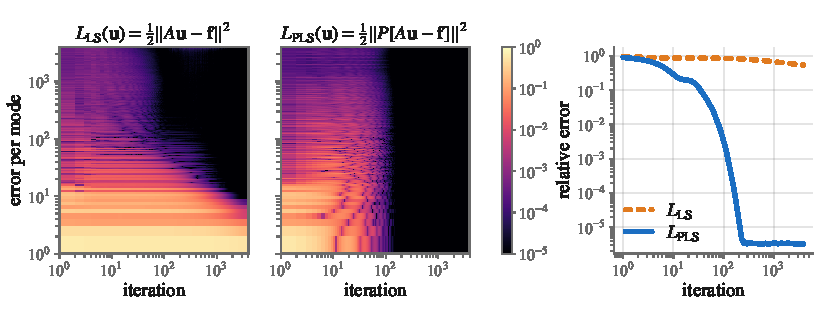
\includegraphics[width=\linewidth]{figures/graphical_abstract.pdf}
   \caption{Ill-conditioning in physics-informed learning: The figure compares Adam minimization of a linear model with and without preconditioning for a physics-informed loss originating from a Poisson problem on a $64^2$ grid. The \textbf{left} and \textbf{centre} report error in each eigenmode of $A$ along the iteration, with the smoothest mode at the bottom. The \textbf{right} figure compares the relative $L^2$ error during training.}
   \label{fig:graphical_abstract}
\end{figure}

% Physics-Informed Training: desirable but presently infeasible (prior to this work)
\paragraph{Physics-Informed Training}

Whenever the governing physics in the form of PDEs are known, neural operators can---in principle---be trained in a self-supervised fashion, relying on the physics residual or variational principles as a loss function. This approach is referred to as \emph{physics-informed neural operator training}, and a natural idea present in the community since the inceptions of neural operators []. However, the success of physics-informed training of neural operators has remained limited to benign equations and learning tasks. More often than not, purely physics-informed learning fails to converge. In fact, supervised learning with its offline data-generation pipeline remains the gold standard for almost all applications. Nevertheless, physics-informed training offers unique advantages, such as the training in the infinite data-limit, where no sample is revisited, and, of course, it removes the need of an expensive dataset generation process.

% We identify the culprit that has prevented physics-informed neural operator learning
\paragraph{Ill-Conditioning of PDE Operators}
In this manuscript, we show that the pathologies of physics-informed neural operator learning can be attributed to a single foundational property of PDE operators: PDE operators are unbounded maps, meaning they magnify their inputs without bounds, and thus lead to severe ill-conditioning in physics-informed loss functions. To make this concrete, take the derivative operator
\begin{equation}\label{eq:derivative_operator}
   \frac{d}{dx}: C^1(0,1) \subset L^2(0,1) \to L^2(0,1), \quad u \mapsto u',
\end{equation}
which amplifies oscillations: $x\mapsto \sin(\omega x)$ is bounded in $L^2(0,1)$ independent of $\omega \in \mathbb R$, but its derivative $x\mapsto \omega \cos(\omega x)$ grows without bound in $L^2(0,1)$ when $\omega \to \infty$. This phenomenon is inherent in all PDE operators. In the case of Poisson's equation, and for a linear model that is the linear combination of a given basis set $\phi_1, \dots, \phi_n$, the physics-informed least-squares loss\footnote{If the equation admits, energy formulations (variational principles) are an attractive alternative.} on a single data point $f$ takes the form
\begin{equation}\label{eq:physics_informed_ls_loss_no_precond}
   L_{\textup{LS}}(u) = \frac12 \| Au - f \|^2, \quad A_{ij} = \int_\Omega \nabla \phi_j \nabla \phi_i\,\mathrm dx,
\end{equation}
where $A\in\mathbb R^{N\times N}$ is the stiffness matrix. The condition number of $A$ scales like $h^{-2}$ for standard bases, where $h$ is the characteristic mesh-size. Conditioning thus deteriorates under mesh refinement, as higher oscillating frequencies can be resolved, the same manifestation of the unbounded nature of PDE operators stressed in \ref{eq:derivative_operator}. Note tha $\nabla^2L_{\textup{LS}} = A^2$, hence the condition number governing the convergence speed of gradient descent (GD) scales like $h^{-4}$. Figure \ref{fig:graphical_abstract} illustrates that this ill-conditioning is so severe that training with first-order methods like GD and Adam becomes infeasible already for very coarse meshes, even in the benign case of a linear ansatz (no neural network at all). In the remainder of this article, we show that precisely this ill-conditioning renders physics-informed neural operator learning infeasible.

\paragraph{Preconditioned Physics-Informed Training}

To counter the ill-conditioning of the least-squares loss \eqref{eq:physics_informed_ls_loss_no_precond}, we rely on \emph{preconditioning}---precisely the tool the numerical analysis community uses to efficiently employ iterative methods in ill-conditioned settings in classical scientific computing. Abstractly, we \emph{modify the least-squares loss} to include an invertible preconditioner $P$ and a positive definite and symmetric weighting matrix $B$
\begin{equation}\label{eq:preconditiones_least_squares_loss}
   L_{\textup{PLS}}(u) = \frac12 \| P[Au - f] \|_B^2,
\end{equation}
We stress that this construction is agnostic to the neural operator architecture employed and adds zero overhead to the inference once training finishes as it only influences the loss function. On a conceptual level, the preconditioned loss \eqref{eq:preconditiones_least_squares_loss} changes the norm in which the error is measured. For any given $P$ we can recast the 
\begin{equation*}
   L_{\textup{PLS}}(u) 
   =
   \frac12 \| P[Au - f] \|_B^2 
   =
   \frac12(PAe, PAe)_B
\end{equation*}
with the error $e=u - A^{-1}f$. This means $P$ maps $Ae$ into a different space and thereby improves conditioning, and $B$ measures the error in this space in an appropriate manner. The choice $P=A^{-1}$ and $B=I$\footnote{Or alternatively, $B=M$, where $M$ is the mass matrix.} recovers data-driven training and reduces the condition number of $\nabla^2L_{\textup{PLS}}$ to unity. In practice, this is realized through fast approximate inverses $P\approx A^{-1}$, e.g., via multigrid methods []. Note that $P\approx A^{-1}$ is not the only choice; for saddle point problems, we alternatively employ block-diagonal preconditioners. Additionally, whenever applicable, we investigate energy formulations, as these are naturally less ill-conditioned.

\subsection{Main Contributions} The main contributions are
\begin{itemize}
   \item \textbf{Efficient physics-informed neural operator training.} We demonstrate that preconditioned physics-informed neural operator training allows data-free training of neural operators at comparable cost and accuracy of the gold standard of data-driven training. Our approach vastly outperforms previous approaches and is demonstrated for the Poisson, Allen-Cahn, and Stokes equation.
   \item \textbf{Flexibility and inference speed.} Our method can be combined with any neural operator architecture and once trained, adds no additional cost to the inference.
   \item \textbf{Training at infinite data limit.} Physics-informed training allows to practically approximate the infinite data limit, where no sample is visited twice. We demonstrate empirically that this is a favorable training paradigm for neural operators.
\end{itemize}

\subsection{Related Literature}
\begin{itemize}
    \item Discussion of physics-informed training in general, in particular for PINNs and NQS.
    \item Paper of Wolfgang and Markus on preconditioning.
    \item OG paper on physics-informed neural operators.
    \item Papers on suboptimal fixes for physics-informed neural operator training.
\end{itemize}

\section{Physics-Informed Training of Neural Operators}

Our goal is to approximate an operator $\mathcal G:\mathcal F \to \mathcal U$ between function spaces $\mathcal U$ and $\mathcal F$. We aim to approximate $\mathcal G$ by a neural network $\mathcal G \approx \mathcal G_\theta$. Neural operators are a special class of neural networks well-suited to the infinite-dimensional nature of the function spaces appearing in PDE applications. However, the concrete neural network structure of $\mathcal G_\theta$ is secondary for our proposed training methodology. A simple but crucial observation we make, is that we can always write the neural operator output in the \emph{interpolated form} %I want this representation to get a name
\begin{equation}\label{eq:neural_operator_interpolated_form}
   \mathcal G_\theta(f) = \sum_{i=1}^n \mathbf{u}(\theta, f)_i \phi_i,
\end{equation}
where $\mathbf u(\theta, f)\in\mathbb R^n$ are coefficients depending on the trainable weights and the functional input $f$. The functions $\phi_1, \dots,\phi_n$ are a fixed basis and span a finite-dimensional function space $\mathcal U_h$, where $h$ denotes a characteristic mesh-size\footnote{Or more general, a quantification of how ``fine'' the space $\mathcal U_h$ is.}. Typical choices are finite element spaces, like piecewise polynomial spaces on a triangulated computational domain. It is crucial to stress that $\phi_1,\dots, \phi_n$, and thus $\mathcal U_h$ is a modeling choice, and a standard neural operator architecture will not automatically map into $\mathcal U_h$. However, we can always interpolate into $\mathcal U_h$. This is a typically sparse, non-trainable operation that adds negligible computational overhead and we will from now on assume that our neural operator is the form described in \eqref{eq:neural_operator_interpolated_form}.

\subsection{Physics-Informed Loss Functions}
For simplicity of exposition, we will work in the setting of linear PDEs that can be formulated in terms of bilinear forms, and we will restrict the discussion to learning the solution operator of such PDEs, although our experimental evaluation is broader. The operator learning problem is to find $u\in\mathcal U$ such that for given $f\in\mathcal F$ it holds
\begin{equation}\label{eq:weak_formulation}
   a(u,v) = f(v), \quad \text{for all }v\in\mathcal U.
\end{equation}
Here, $a$ is a bounded and symmetric bilinear form on $\mathcal U$, and the setting implies $\mathcal F=\mathcal U^*$. We assume all spaces to be Hilbert spaces. The solution operator is $\mathcal G:f\mapsto u$, where $u$ solves \eqref{eq:weak_formulation}. The weak equation can be written as a matrix equation, once $u$ is approximated in $\mathcal U_h$, and takes the form
\begin{equation*}
   A\mathbf u = \mathbf f, \quad \text{with }A_{ij} = a(\phi_j, \phi_i), \quad \mathbf f_i=f(\phi_i).
\end{equation*}
From this equation, we derive the single sample physics-informed loss function via a least-squares construction
\begin{equation}\label{eq:LS_loss_in_theta}
   L_{\textup{LS}}(\theta) = \frac12 \| A \mathbf u(\theta, f) - \mathbf f \|^2.
\end{equation}
For analysis purposes, we will frequently ignore the nonlinear parametrization $\mathbf u(\theta, f)$ and work in the Euclidean space of $\mathbf u\in\mathbb R^n$ directly. We indicate this by writing $L_{\textup{LS}}(u) = \frac 12 \| A\mathbf u - \mathbf f \|^2$ with the understanding that everything is in the variable $\mathbf u$.
% \begin{equation}\label{eq:LS_loss_in_u}
%    L_{\textup{LS}}(u) = \frac 12 \| A\mathbf u - \mathbf f \|^2
% \end{equation}
If $a$ is coercive and symmetric, an energy formulation is an attractive alternative to \eqref{eq:weak_formulation}. In this case, we can find the solution $u$ via a variational principle as the minimizer of the energy $\tfrac12 a(v,v)-f(v)$. The loss function to train the neural operator is, again on a single sample
\begin{equation}
   L_{\textup{Var}}(\theta)= \frac12 \mathbf u(\theta, f)^\top A \mathbf u(\theta, f) - \mathbf f^\top \mathbf u(\theta, f).
\end{equation}


\subsection{Preconditioning} %state convergence result of GD to illustrate why ill-conditioning is relevant?
The least-square loss \ref{eq:LS_loss_in_theta}, although faithfully recovering the solution of $A\mathbf u = \mathbf f$ whenever $A$ is bijective, is unworkable in practice due to its ill-conditioning. This can be seen by computing the Hessian $\nabla_u^2 L_{\textup{LS}}=A^\top A$. In the representative scenario of the Poisson equation [], the condition number $\kappa(A^\top A)$ scales like $h^{-4}$, and makes iterative methods inefficient or, due to round-off errors, entirely useless. To counter this effect, we propose the preconditioned least-squares loss
\begin{equation}
   L_{\textup{PLS}}(u) = \frac12 \| P[A\mathbf u - \mathbf f] \|_B^2,
\end{equation}
where $P\in\mathbb R^{n\times n}$ is an invertible matrix, and $B\in\mathbb R^{n\times n}$ is symmetric and positive definite, hence induces an inner product. The choice of $P$ and $B$ is intuitively coupled: $P$ transforms the range space of $A$ thereby improving conditioning, and $B$ should induce a meaningful norm on the transformed space. To assess conditioning of $L_{\textup{PLS}}$, we compute the Hessian with respect to $\mathbf u$
\begin{equation}
   \nabla^2_u L_{\textup{PLS}}(u) = A^\top P^\top B P A.
\end{equation}
We discuss a few choices of $P$ and $A$.

\subsubsection{Approximate Inverse Preconditioners} We refer to the choice $P\approx A^{-1}$ and $B=I$ or a similarly well-conditioned matrix, like the mass matrix $M_{ij}=(\phi_i,\phi_j)_{L^2}$ as the approximate inverse setting. As proven in Lemma [] in the Appendix, this yields
\begin{equation*}
   \kappa(PA)^2 
   \approx
   \frac{\kappa(PA)^2}{\kappa(B)}
   \leq
   \kappa(A^\top P^\top B P A) 
   \leq 
   \kappa(PA)^2\kappa(B)
   \approx 
   \kappa(PA)^2
\end{equation*}
and in the case of a well conditioned matrix $B$, the conditioning is determined by the accuracy of the approximation $P\approx A^{-1}$. The approximate inverse setting is only practical when the application of $P$ is computationally efficient. For elliptic equations, multigrid methods provide such a preconditioner $P$ at the optimal complexity $\mathcal O(n)$, see [].

\subsubsection{Block-diagonal Preconditioners} We assume the following block structure for $A$, $\mathbf u$ and $\mathbf f$
\begin{align*}
   A = 
   \begin{pmatrix}
      K & D^\top \\ 
      D & 0   
   \end{pmatrix},
   \quad
   \mathbf u = 
   \begin{pmatrix}
      \mathbf w \\
      \mathbf p
   \end{pmatrix},
   \quad
   \mathbf f =
   \begin{pmatrix}
      \mathbf g \\
      0
   \end{pmatrix}.
\end{align*}
We assume that $K$ is symmetric and positive definite, and that $D^\top$ is injective. In this situation the symmetric system $A$ is indefinite and invertible---a well-posed discretization of a saddle point problem, as arises from Stokes equation. The Schur complement is $S=DK^{-1}D^\top$, and the classical choice of block-diagonal preconditioner is
\begin{equation*}
   P \approx \operatorname{diag}(K^{-1}, S^{-1}),
\end{equation*}
where in applications the block inverses can frequently be handled by multigrid methods. The key property of the preconditioner is that $PA$ has exactly three eigenvalues $\{ 1, \frac{1+\sqrt 5}{2}, \frac{1-\sqrt 5}{2} \}$. However, $PA$ remains ill-conditioned in Euclidean norm as it is a non-normal matrix, and in particular, $P$ is not an approximate inverse of $A$. To leverage $P$ in the context of the least-squares loss, we use it to measure the norm of the residual (we use it as $B$ in \eqref{eq:preconditiones_least_squares_loss}), i.e., the loss becomes
\begin{equation*}
   \frac{1}{2} \| A\mathbf u - \mathbf f \|^2_P 
   =
   \frac12 \| K\mathbf w + D^\top \mathbf p - \mathbf g \|^2_{K^{-1}} + \frac12 \| D\mathbf p \|^2_{S^{-1}}.
\end{equation*}
As $A$ is symmetric, its Hessian is $APA$, and Lemma [] shows 
\begin{equation*}
   \kappa(APA) \leq \kappa(P)\left(\frac{\max|\lambda(PA)|}{\min|\lambda(PA)|}\right)^2.
\end{equation*}
Hence conditioning is governed by $\kappa(P)$, which is $\mathcal O(h^{-2})$ for the prototypical case of Stokes equation, hence ill-conditioning remains, but is drastically improved from the $\mathcal O(h^{-4})$ scaling without preconditioner. We discuss further preconditioning options with the block-diagonal preconditioner in Appendix [], but stress that all lead to worse outcomes. Finally, we mention that for Stokes equation monolithic multigrid methods exist, and these fall under the approximate inverse setting.

\subsubsection{Preconditioning Energy Formulations}
Whenever the form $a$ is symmetric and coercive, we can use the loss function $L_{\textup{Var}}(\mathbf u) = \tfrac12\mathbf u^\top A \mathbf u - \mathbf f^\top u$. Its Hessian in $\mathbf u$ is
$
   \nabla^2_u L_{\textup{Var}} = A,
$
hence its conditioning is the square root of $L_\textup{LS}$; and in the prototypical setting of the Poisson equation, it is $\mathcal O(h^{-2})$. Under the restrictive assumption that $P$ and $A$ commute and $P$ is symmetric and positive definite, we can define the preconditioned variational loss
\begin{equation*}
   L_{\textup{PVar}}(\mathbf u) = \frac12 (\mathbf u, A \mathbf u)_P - (\mathbf f, \mathbf u)_P.
\end{equation*}
The critical points $\nabla_u L_{\textup{PVar}}(\mathbf u) = 0$ are characterized by $PA\mathbf u = P\mathbf f$, and thus the minimizer of $L_\textup{Var}$ is unchanged under this transformation. The Hessian is
$
   \nabla^2_u L_{\textup{PVar}}(\mathbf u) = PA.
$
Preconditioners that commute with $A$ are e.g. polynomials in $A$ like []. In practice, we \emph{violate the requirement} $PA=AP$ and merely modify the gradient $\nabla_u L_\textup{Var}(\mathbf u) = A\mathbf u - \mathbf f$ to be $P[A\mathbf u - \mathbf f]$ in the backward pass. Empirically, the choice $P\approx A^{-1}$ via a multigrid method performs reasonable although commutativity is not exactly satisfied.

\subsubsection{Preconditioning Through Architecture Modification}
For both $L_{\textup{LS}}$ and $L_{\textup{Var}}$ we can---in principle---achieve preconditioning by a transformation with $P$: $\tilde L_\textup{LS}(\mathbf u) = L_\textup{LS}(P\mathbf u)$. This yields for $B=I$ for simplicity
\begin{equation*}
   \nabla_u^2 \tilde L_{\textup{LS}}(\mathbf u) = P^\top A^\top A P,
\end{equation*}
and similarly $\nabla_u^2 \tilde L_{\textup{Var}}(\mathbf u) = P^\top A P$. However, this construction requires $P$ to be evaluated at inference time as a part of the forward pass of the model, which is why we do not develop this idea further in this manuscript.

\section{Numerical Results}

\subsection{Poisson Equation}
We are interested in approximating the solution operator $\mathcal G$ of the Poisson equation
\begin{align}\label{eq:poisson_equation}
   \begin{split}
      -\Delta u &= f \quad \text{in }\Omega,
      \\
      u &= 0 \quad \text{on }\partial\Omega,
   \end{split}
\end{align}
on the domain $\Omega = [0,1]$ by a Fourier Neural Operator (FNO) $\mathcal G_\theta$. More precisely, $\mathcal G$ maps $f$ to the solution $u$ of \eqref{eq:poisson_equation}. We work on a structured tensor-product grid, and the output of the FNO is interpolated into the space $\mathcal U_h = Q_1^h$ of bilinear quadrilateral finite elements, with (global) basis functions denoted by $\phi_1, \dots,\phi_n$. The corresponding stiffness matrix $A_{ij} = \int_\Omega \nabla \phi_j \nabla \phi_i\,\mathrm dx$ is symmetric and positive definite, which makes both the least-squares formulation and variational formulation available. As an $\mathcal O(n)$ complexity preconditioner $P_{\textup{GMG}}$, we employ a single di-adic V-cycle geometric multigrid method, which falls in the approximate inverse setting []. For details we refer to Appendix [].

\subsubsection{Ill-Conditioning Prevents Physics-Informed Training}
In this experiment, we show that the ill-conditioning of the stiffness matrix $A$ is the reason physics-informed training fails without a preconditioner. To demonstrate this, we use the physics-informed least-squares loss with $B=I$ and a parametrized preconditioner
\begin{equation}
   L^t_\textup{PLS}(\mathbf u) = \frac12 \|P_t[A\mathbf u - \mathbf f] \|^2_2, \quad P_t = (1-t)I + t A^{-1}.
\end{equation}
The preconditioner $P_t$ is a convex mixing between no preconditioning $P_0=I$ and data-driven training $P_1 = A^{-1}$. This pedagogical choice is possible on a small $64\times 64$ grid, and serves to illustrate the effect of preconditioning on the training dynamics. We monitor the relative $L^2(\Omega)$ error averaged over the validation set during training for a number of $t$-values, and compare to the single di-adic V-cycle geometric multigrid preconditioner. The results are reported in Figure [], where we additionally report the condition number of the Hessian $H_t=\nabla_u^2 L_\textup{PLS}^t = AP_t^2A$.

\begin{figure}[t]
  \centering
  % Both authored at exactly 0.49\textwidth (2.695 in) by
  % experiments/poisson/sweep_blend/plot_paper.py, so do not rescale them.
  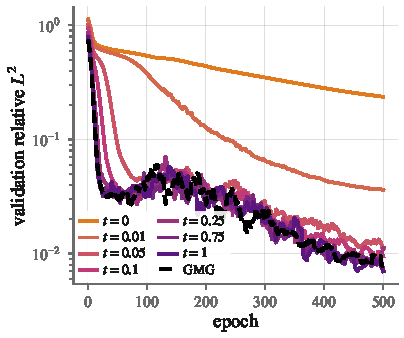
\includegraphics[width=0.49\linewidth]{figures/sweep_overlay.pdf}
  \hfill
  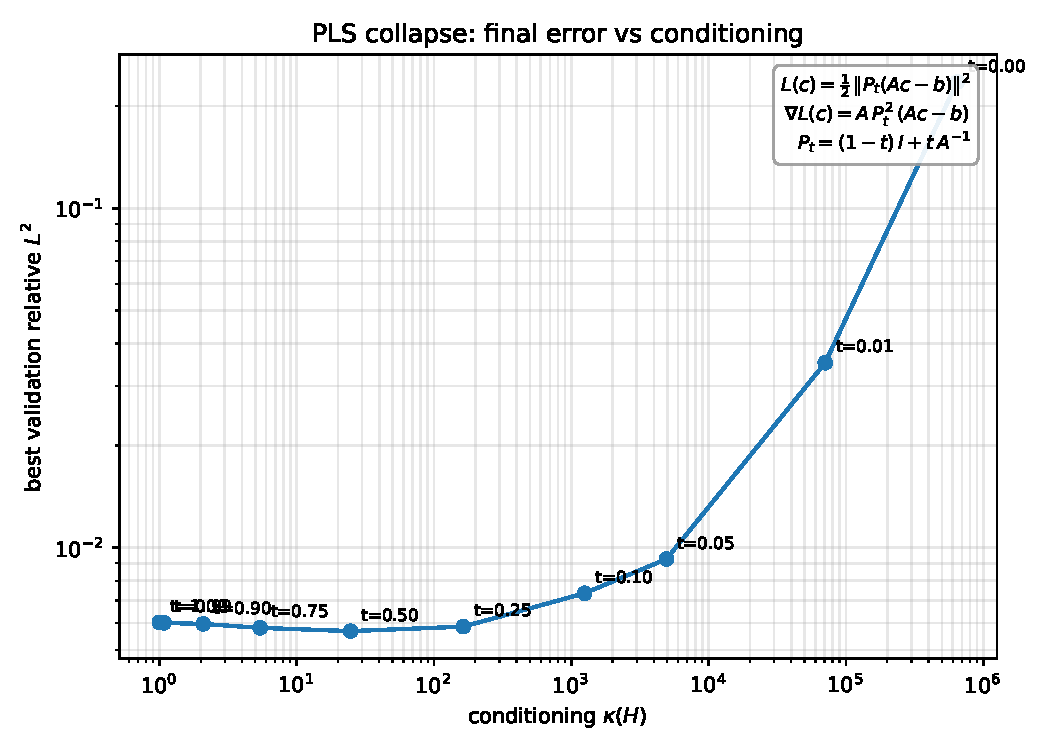
\includegraphics[width=0.49\linewidth]{figures/sweep_collapse.pdf}
  \caption{Preconditioned least-squares training for the Poisson equation. \textbf{Left:} validation relative $L^2$ vs.\ epoch as the preconditioner $P_t$ is swept from $I$ to $A^{-1}$, together with the geometric multigrid preconditioner \textbf{Right:} test error, at the best-validation checkpoint, of the $P_t$ preconditioned sweeps against the condition number $\kappa(H_t)$ of the preconditioned loss Hessian; the dashed line is the geometric multigrid preconditioner, which has no finite $\kappa(H_t)$.}
  \label{fig:pls-overlay}
\end{figure}

\begin{wrapfigure}{r}{0.40\textwidth}
   \vspace{-\intextsep}
   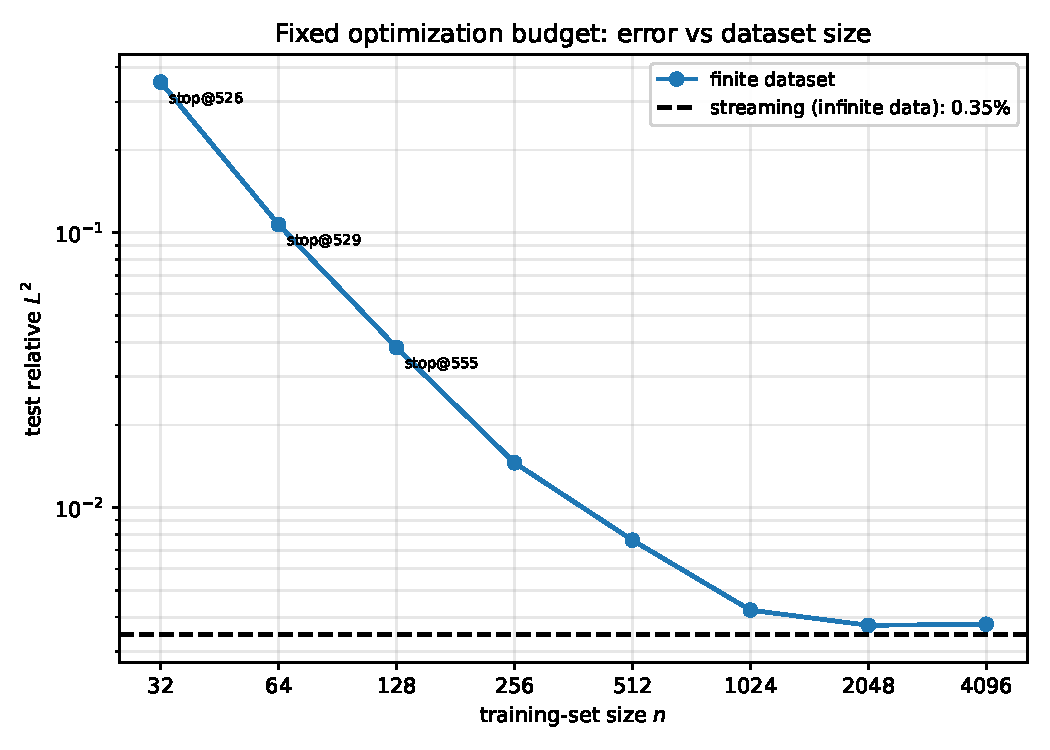
\includegraphics[width=\linewidth]{figures/scaling_test_rl2.pdf}
   \caption{Test error vs.\ dataset size at a fixed budget; dashed is the infinite-data limit.}
   \label{fig:data-scaling}
\end{wrapfigure}
Figure \ref{fig:pls-overlay} shows that that preconditioning is essential to obtain efficient physics-informed training. The un-preconditioned run ($t=0$) converges to $\approx 30\%$ relative $L^2$ error after 500 epochs of training with Adam., while data-driven training ($t=1$) lands at below $1\%$ error for the same amount of training epochs. Intermediate values of $t$ interpolate the training dynamics, which leads us to conclude that ill-conditioning prevents efficient physics-informed neural operator training, and preconditioning is an effective strategy to mitigate this. This is further supported by tracking the condition numbers of $H_t$ in dependence on $t$. For $t=0$, we have $\kappa(H_t)=6.5e+05$ and of course for data-driven training it holds $\kappa(H_1)=1$. Interestingly, as visualized on the right of Figure \ref{fig:pls-overlay} below a conditioning of $approx 10^3-10^4$ (corresponding to $t\in[0.05, 0.1]$) we observe diminishing returns for making the preconditioners more accurate. We attribute this to ill-conditioning induced by the neural network parametrization, which is not resolved in our analysis. This suggests, that a highly-accurate preconditioner may not be needed for accurate physics-informed training, and in fact, the geometric multigrid preconditioner performs virtually identical to the gold standard of data-driven training.

\emph{The deep Ritz results come here, or if space is scarce, we put them in the Appendix. They are nice, but not fundamental.}

\subsubsection{Training at The Infinite Data Limit}
Physics-informed training is not bound to a dataset. Instead, we may draw a fresh batch of samples for every update of the model's parameters. We refer to this as \emph{training at the infinite data limit}. To illustrate the benefit of training in this regime, we fix an optimization budget: 500 epochs' worth of forward passes at a dataset size of 1024 and compare the final relative test $L^2$ error achieved for datasets of growing size, see Figure []. We clearly see the benefit of training in the infinite data regime, even for a fixed finite training budget. 

\subsection{Allen-Cahn Equation}
We now learn a time-increment operator for the Allen-Cahn equation with homogeneous Dirichlet boundary conditions
\begin{align}\label{eq:allen_cahn}
   \begin{split}
      \partial_t u = \Delta u + \varepsilon^2 u(1-u), \quad u_{|\partial\Omega}=0,
   \end{split}
\end{align}
on the domain $\Omega=[0,1]$ and time interval $I=[0,1]$ with $\eps=32$. The Allen-Cahn equation is the $L^2$ gradient flow of the Ginzburg-Landau energy, see Appendix [] for details, and it models phase separation of non-mixing phases. We again use a FNO $\mathcal G_\theta$ and interpolate its output into the space $\mathcal U_h = Q_1^h$ on a tensor-product grid. Discretizing \eqref{eq:allen_cahn} in $Q_1^h$ and employing a convex-concave splitting integrator, the discrete timestep $\mathbf u_{k+1}$ given $\mathbf u_k$ satisfies
\begin{equation}\label{eq:convex_concave_time_stepper}
   0 
   =
   M\left[ \frac{\mathbf u_{k+1} - \mathbf u_k}{\tau} + \varepsilon^2\left( \mathbf u_{k+1}^3 - \mathbf u_k \right) \right]
   +
   A \mathbf u_{k+1}
   =:
   \phi(\mathbf u_{k+1}, \mathbf u_k), 
\end{equation}
where $A_{ij}=\int_\Omega \nabla \phi_j\nabla \phi_i\,\mathrm dx$ is the stiffness matrix, and $M=\int_\Omega \phi_j \phi_i\,\mathrm dx$ is the mass matrix. The scheme \ref{eq:convex_concave_time_stepper} is used to produce a ground truth dataset over a sinusoidal distribution of initial conditions using \texttt{TensorMesh} []. Alternatively, we employ a minimizing movement-type loss that produces $\mathbf u_{k+1}$ from $\mathbf u_k$ as the minimizer
\begin{align}
   \begin{split}
      \mathbf u_{k+1}
      =
      \underset{\mathbf u}{\operatorname{argmin}}\, J(\mathbf u, \mathbf u_k)
      &=
      \frac12\mathbf u^\top A \mathbf u 
      +
      \frac{\eps^2}{4} \mathbf 1^\top M \mathbf u^4 
      -
      \varepsilon^2 \mathbf u_k^\top M \mathbf u 
      \\&+
      \frac{1}{2 \tau}(\mathbf u - \mathbf u_k)^\top M(\mathbf u - \mathbf u_k). 
   \end{split}
\end{align}
We derive $J$ from a variational principle in the Appendix [], note that essentially $\nabla_u J(\mathbf u,\mathbf u_k)=\phi(\mathbf u, \mathbf u_k)$.

\subsubsection{Preconditioned Physics-Informed Training}
Given an initial condition $\mathbf u_0$, we denote the reference roll-out by $\mathbf u_i$, $i=0,\dots,T$ which is produced from \ref{eq:convex_concave_time_stepper} with a finite element method. The roll-out of the FNO is denoted by $\mathcal G_\theta^i(\mathbf u_0)$, and when we write $\hat{\mathbf u}_i$, we mean $\mathcal G_\theta^i(\mathbf u_0)$ with \emph{detached gradients}. The data-driven loss on a single trajectory is
\begin{equation}
   L_{\textup{data}}(\theta) = \frac12 \sum_{k=0}^{R-1}\left\| \mathcal G_\theta(\hat{\mathbf u}_k) - \mathbf u_{k+1} \right\|^2
\end{equation}
where we use $\hat{\mathbf u}_k$ to avoid backpropagation through the graph of $\mathcal G_\theta^k$---the $k$-th power of the FNO and $R\in\mathbb N$ is a hyperparameter of the training setup. The least-squares loss and the minimizing movement loss are
\begin{equation}
   L_{\textup{LS}(\theta)}=\frac12\sum_{k=0}^{R-1}\left\| \phi(\mathcal G_\theta(\hat{\mathbf u}_k), \hat{\mathbf u}_k) \right\|^2, 
   \quad
   L_{\textup{MM}}(\theta) = \sum_{k=0}^{R-1}J(\mathcal G_\theta(\hat{\mathbf u}_k), \hat{\mathbf u}_k)
\end{equation}
\emph{todo: Discuss ill-conditioning.} Finally, we propose a preconditioned variant
\begin{equation}
   L_{\textup{PLS}}(\theta) = \frac12\sum_{k=0}^{R-1}\left\| P[\phi(\mathcal G_\theta(\hat{\mathbf u}_k), \hat{\mathbf u}_k)] \right\|^2,
   \quad
   P\approx \left( (3\varepsilon^2 + \tau^{-1})M + A \right)^{-1}
\end{equation}
which is based on an approximate inverse of the Jacobian $\nabla_u\phi$ and can be realized efficiently via geometric multigrid method.

\subsection{Stokes Equation}

\section{Conclusion}


%Citations within the text should be based on the \texttt{natbib} package
%and include the authors' last names and year (with the ``et~al.'' construct
%for more than two authors). When the authors or the publication are
%included in the sentence, the citation should not be in parenthesis using \verb|\citet{}| (as
%in ``See \citet{Hinton06} for more information.''). Otherwise, the citation
%should be in parenthesis using \verb|\citep{}| (as in ``Deep learning shows promise to make progress
%towards AI~\citep{Bengio+chapter2007}.'').

%The corresponding references are to be listed in alphabetical order of
%authors, in the \textsc{References} section. As to the format of the
%references themselves, any style is acceptable as long as it is used
%consistently.



\subsection*{AI use statement}

(This section is \textbf{required} and does not count toward the page limit.)

% TEMPORARY HOME. Parked here so the figure is not full-width while the Allen-Cahn
% discussion is still empty; move it back into that subsection once there is text to wrap.
\begin{wrapfigure}{r}{0.40\textwidth}
   \vspace{-\intextsep}
   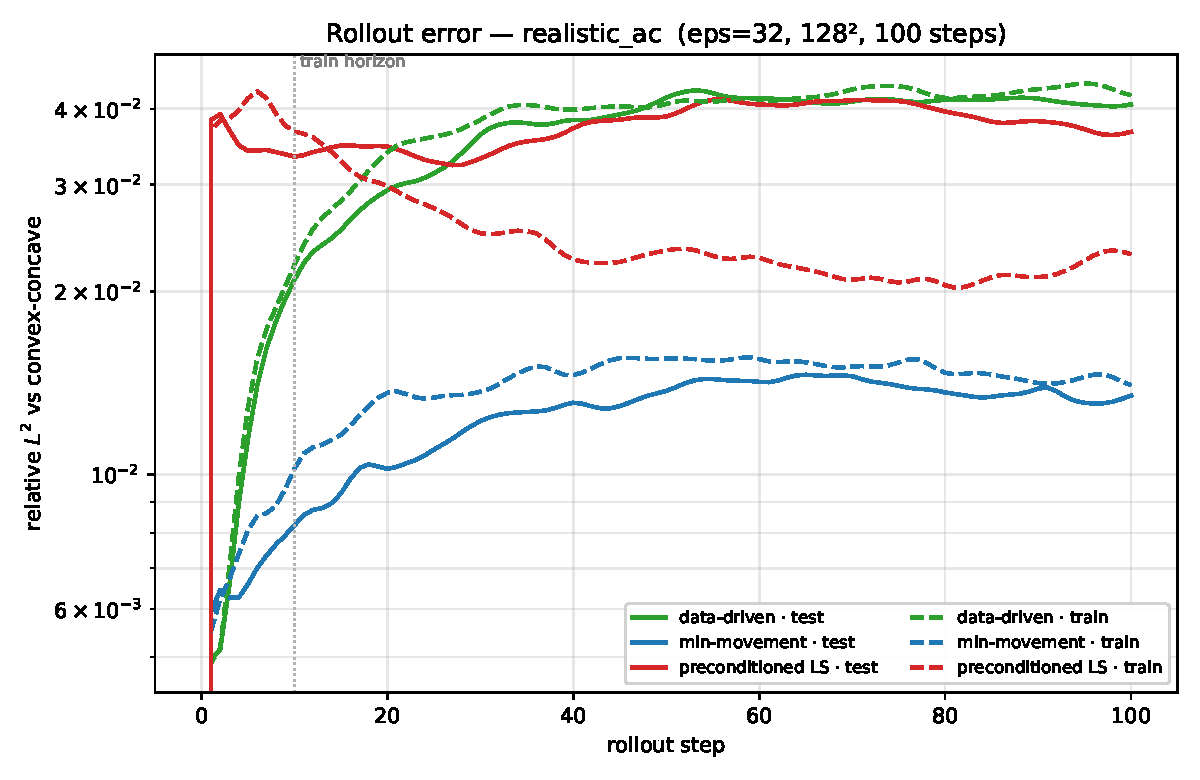
\includegraphics[width=\linewidth]{figures/rollout_error.pdf}
   \caption{Allen-Cahn rollout error vs.\ the convex-concave reference; solid test, dashed train.
   Bare $L_{\textup{LS}}$ collapses and is omitted.}
   \label{fig:ac-rollout}
\end{wrapfigure}
In this work, we used generative AI tools for software implementation and language refinement.
We have not used generative AI tools for drafting the manuscript,
and [the rest of the required disclosure tasks] are not applicable to this work.
Additionally, we used generative AI tools for [tasks with recommended
disclosure]. We have reviewed all AI-assisted work. LLM-generated code was verified and tested for correctness
by the authors. We take responsibility for the final content of this work,
including text, claims or artifacts produced with the aid of generative AI.


\subsection*{Ethics statement}

(This section is \textbf{recommended} and does not count toward the page limit.)

If authors feel that their paper submission raises questions regarding the Code
of Ethics, they are encouraged to include a paragraph of Ethics Statement (at
the end of the main text before references) to address potential concerns where
appropriate. Topics include, but are not limited to, studies that involve human
subjects, practices to data set releases, potentially harmful insights,
methodologies and applications, potential conflicts of interest and sponsorship,
discrimination/bias/fairness concerns, privacy and security issues, legal
compliance, and research integrity issues (e.g., IRB, documentation, research
ethics). This statement should not be more than 1 page.

\subsection*{Reproducibility statement}

(This section is \textbf{recommended} and does not count toward the page limit.)

It is important that the work published in ICLR is reproducible. Authors are
strongly encouraged to include a paragraph-long Reproducibility Statement at the
end of the main text (before references) to discuss the efforts that have been
made to ensure reproducibility. This paragraph should not itself describe
details needed for reproducing the results, but rather reference the parts of
the main paper, appendix, and supplemental materials that will help with
reproducibility. For example, for novel models or algorithms, a link to an
anonymous downloadable source code can be submitted as supplementary materials;
for theoretical results, clear explanations of any assumptions and a complete
proof of the claims can be included in the appendix; for any datasets used in
the experiments, a complete description of the data processing steps can be
provided in the supplementary materials. Each of the above are examples of
things that can be referenced in the reproducibility statement.

\subsubsection*{Author Contributions}
If you'd like to, you may include  a section for author contributions as is done
in many journals. This is optional and at the discretion of the authors.

\subsubsection*{Acknowledgments}
Use unnumbered third level headings for the acknowledgments. All
acknowledgments, including those to funding agencies, go at the end of the paper.


\bibliography{iclr2027_conference}
\bibliographystyle{iclr2027_conference}

\appendix
\section{Appendix}
You may include other additional sections here.


\end{document}
